\documentclass[12pt, a4paper]{article}

% --- Encoding and language ---
\usepackage[utf8]{inputenc}
\usepackage[T1]{fontenc}
\usepackage[provide=*,spanish]{babel}

% --- Math ---
\usepackage{amsmath}
\usepackage{amssymb}

% --- Figures ---
\usepackage{graphicx}
\usepackage{float}
\graphicspath{{figures/}}

% --- Tables ---
\usepackage{booktabs}

% --- Links ---
\usepackage[colorlinks=true, linkcolor=blue, citecolor=blue, urlcolor=blue]{hyperref}

% --- Page layout ---
\usepackage{geometry}
\geometry{margin=2.5cm}

% --- Header/footer ---
\usepackage{fancyhdr}
\setlength{\headheight}{14.5pt}
\addtolength{\topmargin}{-2.5pt}
\pagestyle{fancy}

\fancyhf{}
\rhead{Parcial 1}
\lhead{Thomas Gonzalez}
\cfoot{\thepage}

% ============================================================
\begin{document}

\begin{center}
    {\LARGE\bfseries Parcial 1}\\[0.8em]
    {\large Thomas Gonzalez}\\[0.3em]
    {\normalsize \today}\\[0.4em]
    {\small \href{https://github.com/thomatrixting/Solar_espectrum_analisis}{github del proyecto}}
\end{center}

\vspace{1em}
\hrule
\vspace{1.5em}

% ============================================================
\section{Contexto de los datos utilizados}

Los datos utilizados provienen del instrumento SIM (\textit{Spectral Irradiance Monitor}) a bordo del satélite SORCE (\textit{Solar Radiation and Climate Experiment}) \cite{GESDISCDataseta}. El conjunto de datos contiene mediciones de la irradiancia espectral solar en el rango de 240 a 2413 nm, con una cadencia temporal de 24 horas. Para el análisis se seleccionó la fecha del 27 de octubre de 2006, la cual corresponde al día juliano 2\,454\,036.

% ============================================================
\section{Teoría}

El instrumento SIM reporta el \textbf{flujo monocromático} $F_\lambda$ (denominado irradiancia espectral), definido como la potencia recibida por unidad de área y por unidad de longitud de onda:
\begin{equation}
    [F_\lambda] = \left[\frac{\mathrm{W}}{\mathrm{m}^2\,\mathrm{nm}}\right].
\end{equation}

La \textbf{intensidad específica} $I_\lambda$ se obtiene dividiendo por el ángulo sólido $\Omega_\odot$ subtendido por el Sol:
\begin{equation}
    I_\lambda = \frac{F_\lambda}{\Omega_\odot}
    \quad \left[\frac{\mathrm{W}}{\mathrm{m}^2\,\mathrm{sr}\,\mathrm{nm}}\right],
\end{equation}
donde el ángulo sólido se calcula a partir del radio angular aparente $\alpha$ del Sol:
\begin{equation}
    \Omega_\odot = 2\pi\left(1 - \cos\alpha\right).
\end{equation}

La \textbf{ley de Planck} describe la intensidad específica de un cuerpo negro a temperatura $T$:
\begin{equation}
    B_\lambda(\lambda, T) = \frac{2hc^2}{\lambda^5}
    \frac{1}{\exp\!\left(\dfrac{hc}{\lambda k_B T}\right) - 1},
\end{equation}
donde las constantes $h$, $c$, $k_B$ y $\sigma$ corresponden a los valores directos y derivados (ej: $\sigma$) deCODATA 2014 \cite{mohrCODATARecommendedValues2015} provistos por la librería \texttt{astropy}. Ajustar $B_\lambda(T)$ al espectro observado $I_\lambda$ permite obtener la \textbf{temperatura de color} $T_\mathrm{color}$ del Sol.

Para estimar la \textbf{temperatura efectiva} $T_\mathrm{eff}$, se integra el flujo espectral sobre todo el rango medido y se escala a la superficie solar mediante la ley del inverso del cuadrado:
\begin{equation}
    F_\odot = F_\mathrm{int}\left(\frac{d_\odot}{R_\odot}\right)^2,
\end{equation}
y se aplica la ley de Stefan--Boltzmann:
\begin{equation}
    T_\mathrm{eff} = \left(\frac{F_\odot}{\sigma}\right)^{1/4},
\end{equation}.

% ============================================================
\section{Actividad 1: Flujo monocromático vs.\ longitud de onda}

La figura \ref{fig:flujo} muestra el flujo monocromático $F_\lambda$ en función de la longitud de onda para el 27 de octubre de 2006. Se observa que la distribución espectral se asemeja estrechamente a la de un cuerpo negro de Planck, y que la incertidumbre reportada por el instrumento es despreciable.

\begin{figure}[H]
    \centering
    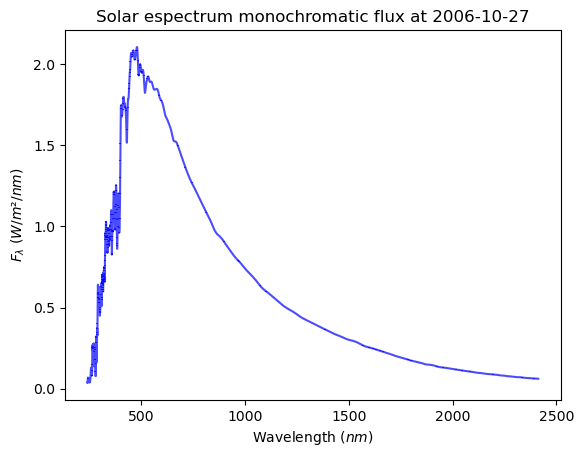
\includegraphics[width=\textwidth]{actividad1_flujo.png}
    \caption{Flujo monocromático solar $F_\lambda$ en función de la longitud de onda para el 27 de octubre de 2006 (SORCE/SIM). Las barras de error son negligibles a esta escala.}
    \label{fig:flujo}
\end{figure}

% ============================================================
\section{Actividad 2: Ángulo sólido del Sol}

A partir de datos de Stellarium para el 27 de octubre de 2006 12:00 UTC se obtuvieron los siguientes parámetros solares:

\begin{center}
\begin{tabular}{ll}
\toprule
Parámetro & Valor \\
\midrule
Radio angular aparente & $0^\circ\,32'\,11.22''$ \\
Distancia Tierra--Sol & $148\,672\,000\ \mathrm{km}$ o $0.994\ \mathrm{UA}$ \\
Unidad astronómica (media) & $149\,597\,870.7\ \mathrm{km}$ \\
Diámetro solar & $1\,392\,000\ \mathrm{km}$ \\
\bottomrule
\end{tabular}
\end{center}

Con el radio angular aparente se calcula el ángulo sólido mediante la ecuación (3):
\begin{equation*}
    \Omega_\odot = 6.886\times10^{-5}\ \mathrm{sr}.
\end{equation*}
Este valor concuerda con el obtenido a partir del radio solar medio y 1 UA ($6.794\times10^{-5}\ \mathrm{sr}$), lo que confirma la consistencia del cálculo. En adelante se utiliza el valor derivado del diámetro angular aparente por ser más preciso para la fecha de observación.

Los efectos de la posición orbital del satélite SORCE son despreciables, pues éste orbita a 569 km de altitud con una inclinación de $40.0^\circ$ y un período de aproximadamente 90 minutos; cualquier variación residual queda promediada por la cadencia de integración de 24 horas.

% ============================================================
\section{Actividad 3: Intensidad específica vs.\ longitud de onda}

Dividiendo $F_\lambda$ por el ángulo sólido $\Omega_\odot$ calculado en la actividad anterior se obtiene la intensidad específica $I_\lambda$, cuya distribución espectral se muestra en la figura \ref{fig:intensidad}.

\begin{figure}[H]
    \centering
    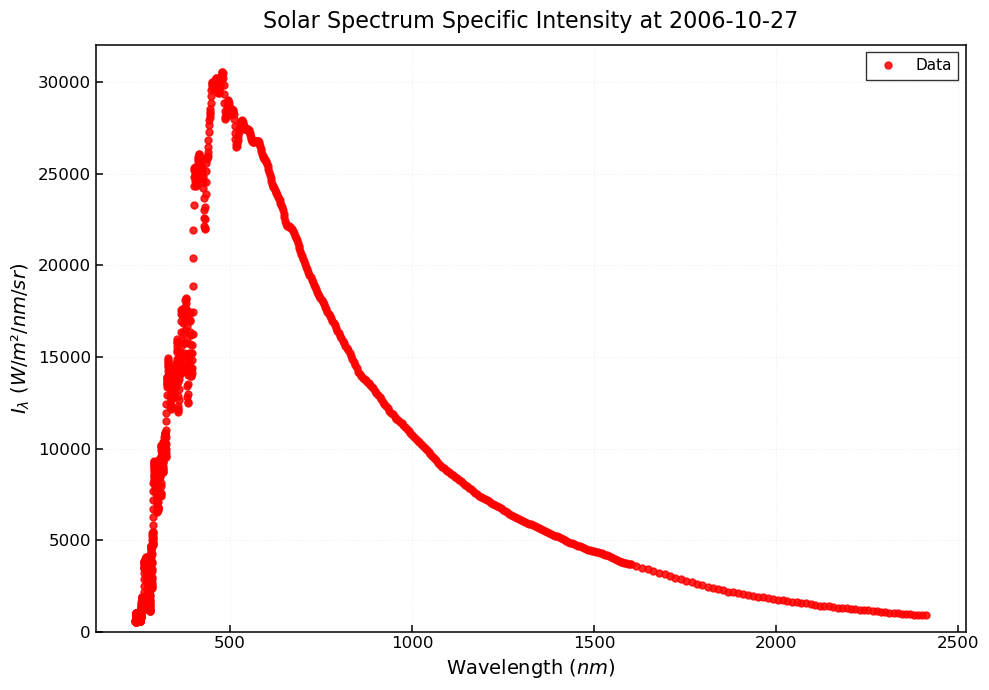
\includegraphics[width=\textwidth]{actividad3_intensidad.png}
    \caption{Intensidad específica solar $I_\lambda$ en función de la longitud de onda para el 27 de octubre de 2006.}
    \label{fig:intensidad}
\end{figure}

% ============================================================
\section{Actividad 4: Ajuste de la curva de Planck --- temperatura de color}

Se superpusieron curvas de Planck a distintas temperaturas sobre el espectro de intensidad específica. Los criterios de ajuste requieren que la curva teórica: (i) tenga su máximo lo más cercano posible al máximo observado, y (ii) cruce al menos un punto experimental antes y despues del máximo. La figura \ref{fig:planck} muestra el proceso de refinamiento progresivo del ajuste.

\begin{figure}[H]
    \centering
    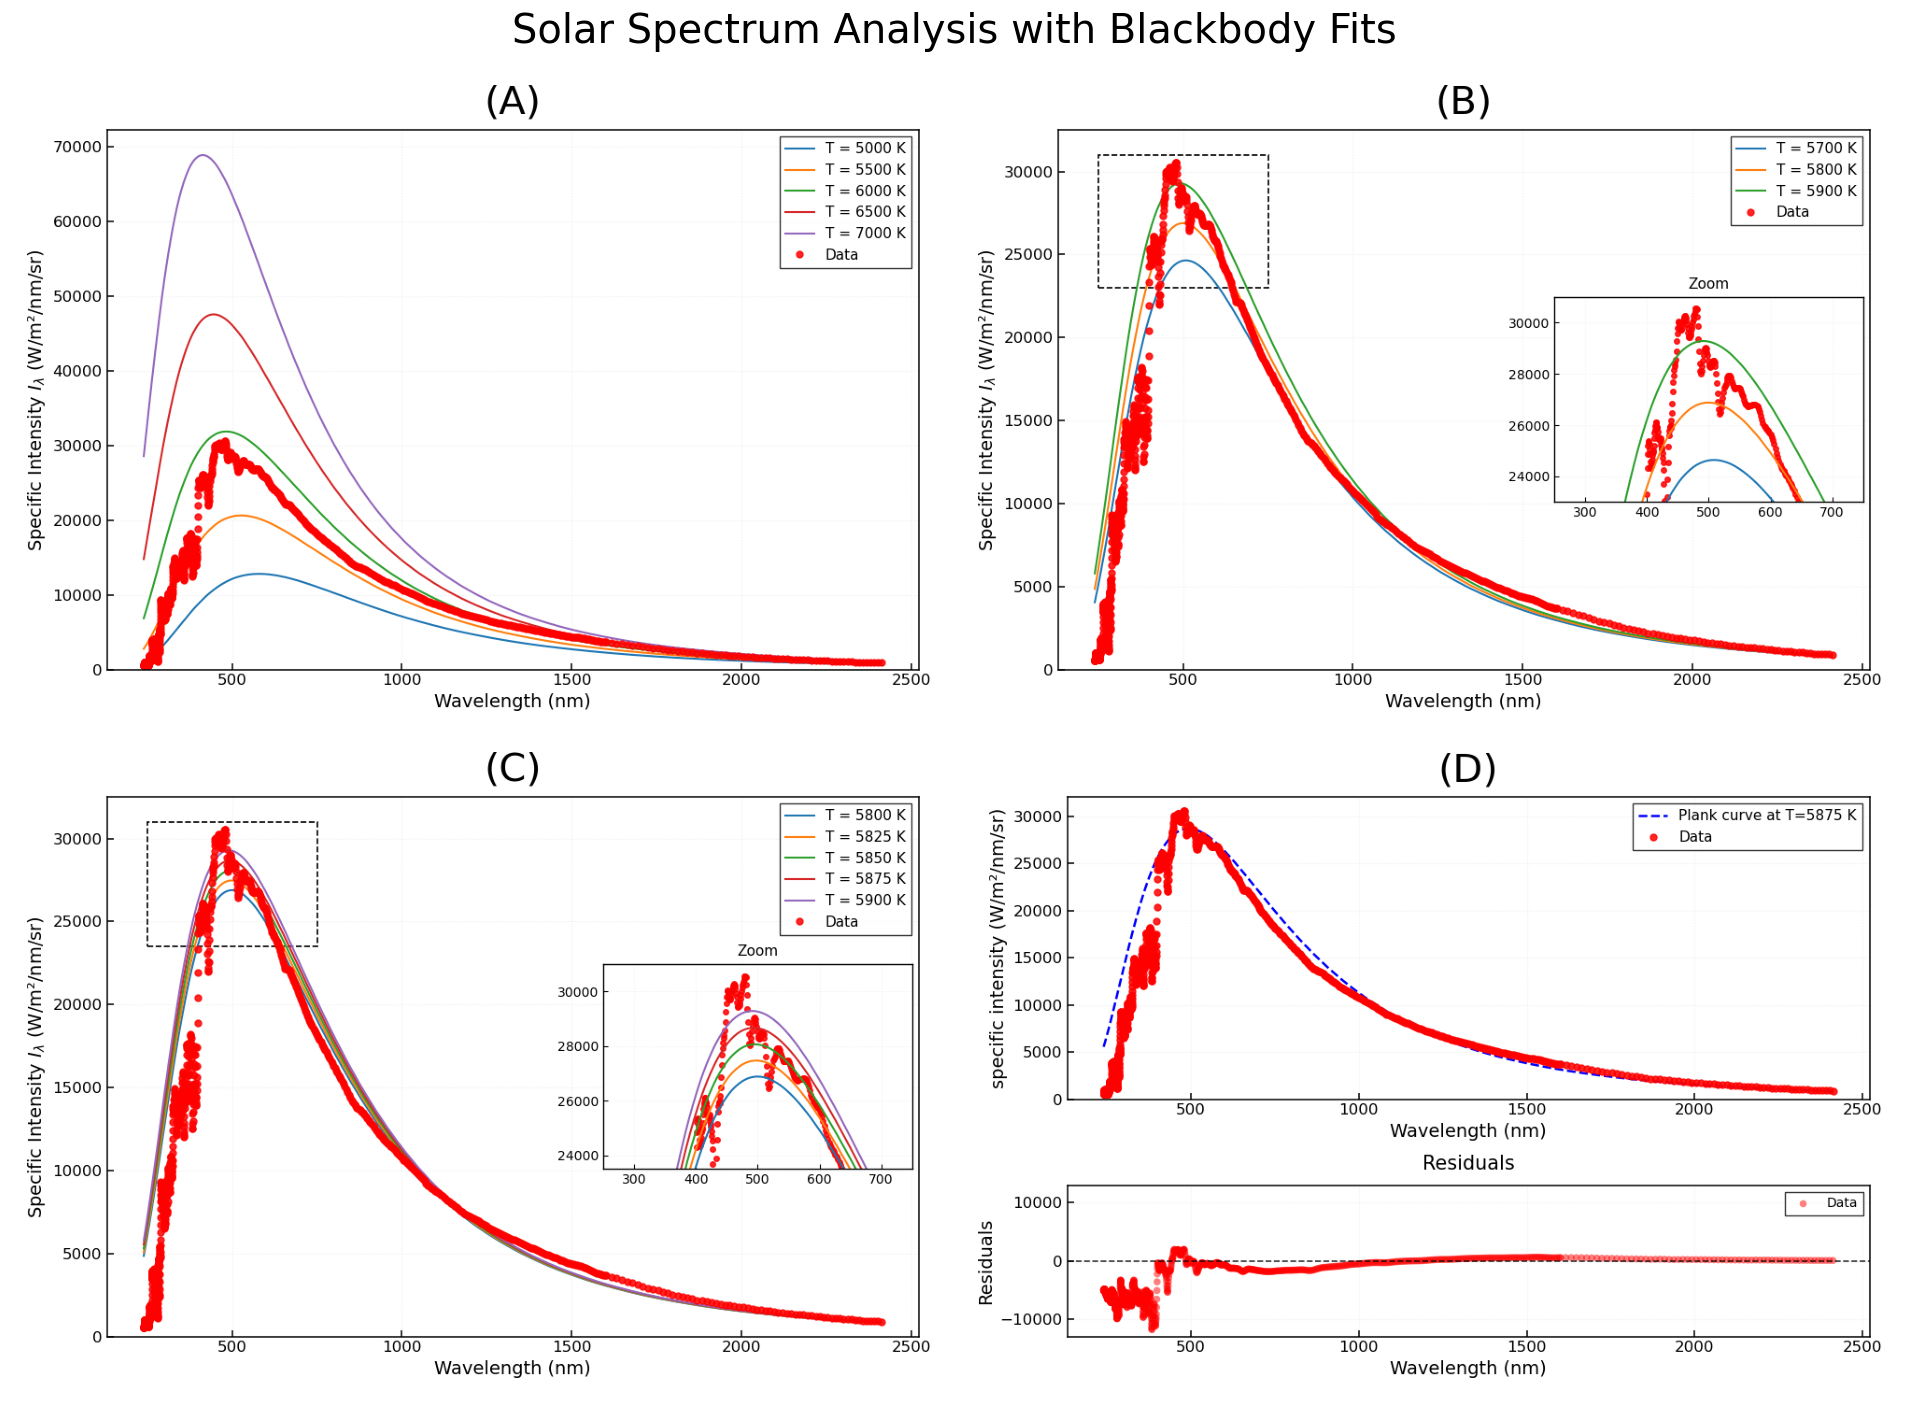
\includegraphics[width=\textwidth]{actividad4_planck_fit.png}
    \caption{Ajuste de curvas de Planck al espectro de intensidad específica. Los paneles (A), (B) y (C) muestran una búsqueda amplia de temperatura; el panel (D) ilustra el ajuste final con residuales normalizados.}
    \label{fig:planck}
\end{figure}

El analisis muestra que la temperatura debe estan entre $5500K$ y $6000K$ (A), posteriormente en (B) se nota que curvas por encima de 5900 K se acercan más al máximo observado, pero no intersectan ningún punto experimental previo al máximo, incumpliendo el segundo criterio. La temperatura que mas se aproxima al maximo y intersecta un punto experimental antes del máximo, como se ve en (C), es:
\begin{equation*}
    T_\mathrm{color} = 5875\ \mathrm{K}.
\end{equation*}
El panel (D) muestra que este ajuste reproduce razonablemente bien el espectro observado; los residuales son atribuibles al ruido inherente a las mediciones del instrumento SIM y al hecho de que se esta aproximando la emision con la de un cuerpo negro.

% ============================================================
\section{Actividad 5: Integración espectral --- temperatura efectiva}

El flujo integrado se obtiene aplicando la regla del trapecio sobre $F_\lambda$ en todo el rango espectral medido, y se corrige por la distancia Tierra--Sol en la fecha de análisis ($r = 0.994\ \mathrm{AU}$) mediante la ley del inverso del cuadrado ($F \propto r^{-2}$):
\begin{equation*}
    F_\mathrm{calc} = 1337.9\ \mathrm{W\,m^{-2}}.
\end{equation*}
Este valor es consistente con el reportado oficialmente por el instrumento SORCE/TIM para la misma fecha:
\begin{equation*}
    F_\mathrm{TIM} = 1360.8\ \mathrm{W\,m^{-2}}.
\end{equation*}
La pequeña discrepancia se debe a que el TIM integra rangos espectrales adicionales no cubiertos por el SIM; dado que la diferencia es menor al 2\%, no se requiere ninguna corrección adicional.

Escalando el flujo integrado a la superficie solar mediante las ecuaciones (5) y (6), se obtiene la temperatura efectiva:
\begin{equation*}
    T_\mathrm{eff} = 5747.1\ \mathrm{K}.
\end{equation*}
Este resultado concuerda razonablemente con la temperatura de color obtenida en la actividad anterior ($T_\mathrm{color} = 5875\ \mathrm{K}$) y con el valor de referencia de $5778\ \mathrm{K}$ reportado en la literatura \cite{stix2002}. La estimación por integración espectral resulta ligeramente más precisa, ya que la integración trapezoidal es más robusta al ruido espectral que un ajuste visual de la curva de Planck.

% ============================================================
\bibliographystyle{plain}
\bibliography{bibliography}

\end{document}
